\documentclass{article}
\usepackage[margin=1in]{geometry}
\usepackage{amsmath,amsthm,amssymb}
\usepackage{bbm,enumerate,mathtools}
\usepackage{tikz,pgfplots}
\usepackage{chessboard}
\usepackage[hidelinks]{hyperref}
\usepackage{multicol} % Problem 35
\usepackage{xstring} % Difficulty command
\usetikzlibrary{shapes.geometric}

\newenvironment{question}{\begin{trivlist}\item[\textbf{Question.}]}{\end{trivlist}}
\newenvironment{note}{\begin{trivlist}\item[\textbf{Note.}]}{\end{trivlist}}
\newenvironment{references}{\begin{trivlist}\item[\textbf{References.}]}{\end{trivlist}}
\newenvironment{related}{\begin{trivlist}\item[\textbf{Related.}]\end{trivlist}\begin{enumerate}}{\end{enumerate}}

\newcommand\score[1]{
\pgfmathsetmacro\pgfxa{#1+1}
\tikzstyle{scorestars}=[
  star,
  star points=5,
  star point ratio=2.25,
  draw,
  inner sep=3pt,
  anchor=outer point 5
]
  \begin{tikzpicture}[baseline]
    \draw[opacity=0] (0,-0.5) rectangle (0,0.2); % Workaround for whitespace at the bottom.
    \foreach \i in {1,...,4} {
      \pgfmathparse{(\i<=#1?"yellow":"gray")}
      \edef\starcolor{\pgfmathresult}
      \draw (\i*4.5ex,0) node[name=star\i,scorestars,fill=\starcolor]  {};
    }
  \end{tikzpicture}
}

\newcommand{\difficulty}[1]{%
  \IfEqCase{#1}{%
      {1}{
        
\begin{tikzpicture}[scale=0.7, baseline=0.9mm]%
          \definecolor{slopegreen}{rgb}{0.0, 0.5, 0.0}%
          \fill[slopegreen] (0.5,0.5) circle (0.5);%
        \end{tikzpicture}%
      }%
      {2}{
        
\begin{tikzpicture}[scale=0.7, baseline=0.9mm]%
          \definecolor{slopeblue}{rgb}{0.0, 0.44, 1.00}
          \fill[slopeblue] (0,0) rectangle (1,1);%
        \end{tikzpicture}%
      }%
      {3}{
\begin{tikzpicture}[scale=0.7, baseline=0.9mm]\fill (0,0.5)--(0.5, 0)--(1,0.5)--(0.5,1)--cycle; \end{tikzpicture}}%
      {4}{
\begin{tikzpicture}[scale=0.7, baseline=0.9mm]\fill (0.25,0)--(0,0.5)--(0.25,1)--(0.5,0.5)--cycle; \fill (0.75,0)--(0.5,0.5)--(0.75,1)--(1,0.5)--cycle;\end{tikzpicture}}%
      % you can add more cases here as desired
  }[\PackageError{difficulty}{Undefined difficulty level: #1}{}]%
}%
\newcommand{\rating}[2]{\difficulty{#1}\\\score{#2}\\}


\begin{document}

\rating{2}{2}
Consider the graded poset on $\mathbb{N}_{>0}$ given by covering relations
$\displaystyle n - \frac{n}{p} \lessdot n$ for all primes $p \mid n$.
\begin{figure}[ht!]
  \centering
  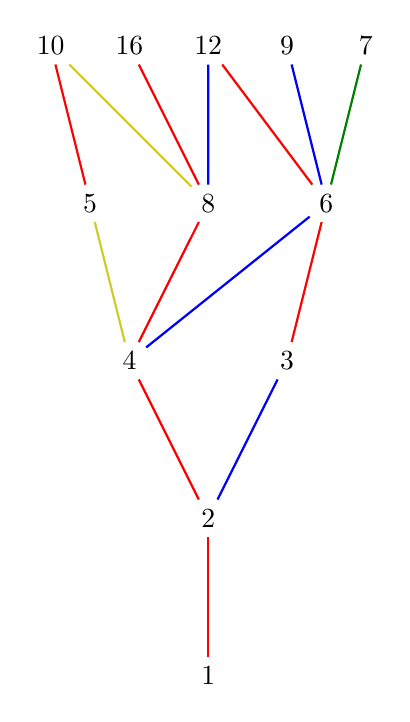
\begin{tikzpicture}
    % Rank 0
    \node (1) at (0,0) {$1$};
    % Rank 1
    \node (2) at (0,2) {$2$};
    % Rank 2
    \node (3) at (1,4) {$3$};
    \node (4) at (-1,4) {$4$};
    % Rank 3
    \node (5) at (-1.5,6) {$5$};
    \node (6) at (1.5,6) {$6$};
    \node (8) at (0,6) {$8$};
    % Rank 4
    \node (7) at (2,8) {$7$};
    \node (9) at (1,8) {$9$};
    \node (10) at (-2,8) {$10$};
    \node (12) at (0,8) {$12$};
    \node (16) at (-1,8) {$16$};

    % Edges
    \draw[thick, red] (1)--(2);

    \draw[thick, blue] (2)--(3);
    \draw[thick, red] (2)--(4);

    \draw[thick, blue] (4)--(6);
    \draw[thick, yellow!80!black] (4)--(5);
    \draw[thick, red] (3)--(6) (4)--(8);

    \draw[thick, blue] (6)--(9) (8)--(12);
    \draw[thick, yellow!80!black] (8)--(10);
    \draw[thick, green!50!black] (6)--(7);
    \draw[thick, red] (5)--(10) (6)--(12) (8)--(16);
  \end{tikzpicture}
  \caption{Ranks $0$ through $4$ of the poset.
  Prime divisors $2, 3, 5,$ and $7$ are displayed as red, blue, gold, and green
  respectively.
  For example, $\displaystyle 12 \gtrdot 12 - \frac{12}{3} = 8$.}
\end{figure}

\begin{question}
  Is this poset a lattice?
\end{question}

\begin{related}
  \item If not, is this poset a join- or meet-semilattice?
  \item If so, is this poset a distributive lattice? A modular lattice?
  \item It appears that (at least for small values of $n$ and $k$)
    $(n \vee k) \mid \operatorname{lcm}(n,k)$.
    What is $\displaystyle \frac{\operatorname{lcm}(n,k)}{n \vee k}$?
  \item Is there a good way to construct the least integer (in the usual sense)
    for a given rank number?
\end{related}

\begin{references}
  \item \url{https://math.stackexchange.com/q/3632156/121988}
  \item \url{https://oeis.org/A334230}
\end{references}
\end{document}
